\textbf{Равномерное распределение}. Говорят, что $\xi$ имеет равномерное распределение на отрезке $[a, b]$ ($\xi \in U_{a,b}$), если плотность распределения $\xi$ постоянна на отрезке $[a, b]$ и равна нуля вне него:
\begin{equation*}
    f_\xi (x) = \left\{\begin{aligned}
        &(b-a)^{-1}, &x\in[a, b], \\
        &0, &x\notin[a, b]. \\
    \end{aligned}\right.
\end{equation*}
Площадь под графиком этой функции равна единице, $f_\xi \geq 0$, так что $f_\xi (x)$ действительно плотность.

Легко теперь посчитать функцию распределения величины $\xi$:
\begin{equation*}
    F_\xi (x) = \P (\xi < x) = \int_{-\infty}^{x} f_\xi (t) \d t = \left\{\begin{aligned}
        &0, & x < a; \\
        & \frac{x-a}{b-a}, & a \leq x \leq b, \\
        &1, &x > b,
    \end{aligned}\right.
\end{equation*}
что вполне логично. График функции распределения и плотности распределения приведен ниже.

\begin{figure}[ht]
    \centering
    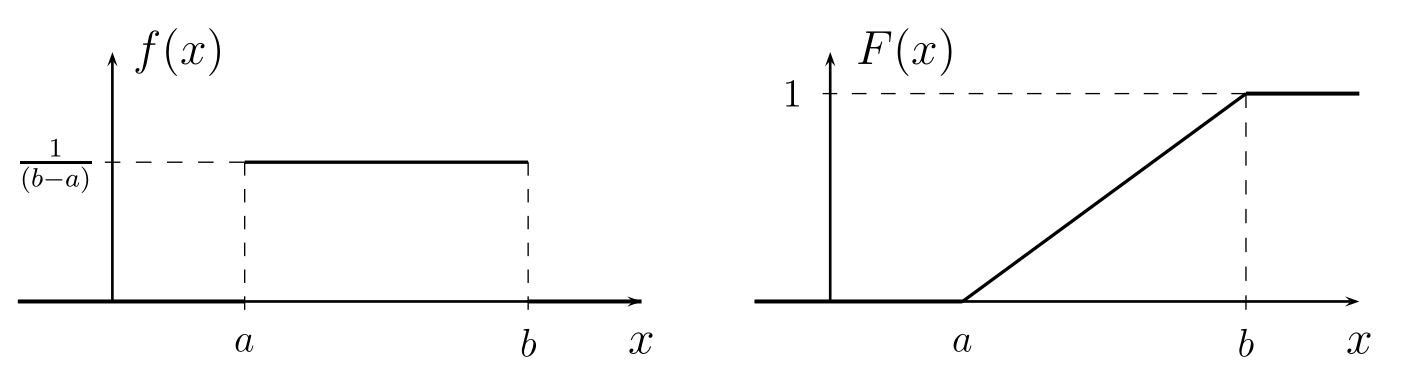
\includegraphics[width=0.5\textwidth]{img/d1.png}
    \caption{ Плотность и функция распределения $U_{a, b}$}
\end{figure}


\textbf{Показательное распределение}.
Говорят, что $\xi$ имеет показательное (экспоненциальное) распределение с параметром $\alpha > 0$ ($\xi \in \textnormal{E}_\alpha$), если $\xi$ имеет следующую плотность распределения:
\begin{equation*}
    f_\xi (x) = \left\{\begin{aligned}
        &0, &x < 0, \\
        \alpha e^{- \alpha x}, & x \geq 0.        
    \end{aligned}\right.
\end{equation*}
Функция распределения случайной величины $\xi$ непрерывна:
\begin{equation*}
    F_\xi (x) = \P (\xi < x) = \left\{\begin{aligned}
        &0, & x < 0, \\
        &1-e^{-\alpha x}, & x \geq 0.
    \end{aligned}\right.
\end{equation*}
Стоит заметить, что показательное распределение является единственным абсоютно непрерывным распределением, для которого выполнено свойство <<нестарения>> (а-ля геоетрическое):

\begin{to_thr}[]
    Пусть $\xi \in \textnormal{E}_\alpha$. Тогда для любых $x, \ y > 0$ верно, что
    $\P(\xi > x + y \mid \xi > x) = \P(\xi > y)$.
\end{to_thr}


\textbf{Нормальное распределение}. Говорят, что $\xi$ имеет \textit{нормальное} (\textit{гауссовское}) распределение с параметрами $a, \, \sigma^2$, где $a \in \mathbb{R}$, $\sigma > 0$ ($\xi \in \textnormal{N}_{a, \sigma^2}$), если $\xi$ имеет плотность распределения вида
\begin{equation}
    f_\xi (x) = \frac{1}{\sigma \sqrt{2 \pi}} \, \exp \left(
        - \frac{(x-a)^2}{2 \sigma^2}
    \right), 
    \hspace{5 mm}
    x \in \mathbb{R}. 
\end{equation}
Это действительно функция распределения, ведь вспоминая интеграл Пуассона
\begin{equation*}
    I = \int_{-\infty}^{+\infty} e^{-x^2/2} \d x = \sqrt{2 \pi},
\end{equation*}
нетрудно заменой переменных свести $\int f_\xi (x) \d x$ к $I$.

\begin{to_def}
    Нормальное распределение $\textnormal{N}_{0, 1}$ называется \textit{стандартным нормальным} распределением.
\end{to_def}

Для функции распределения нормального закона $\textnormal{N}_{a, \sigma^2}$ далее будет использоваться $\Phi_{a, \sigma^2} (x)$ для функции распределения нормального закона $N_{a, \sigma^2}$. 


% \textbf{Гамма-распределение}. Говорят, что $\xi$ имеет гамма-распределение, с параметрами $\alpha > 0$, $\lambda > 0$, 
\textbf{Распределение Коши}. Говорят, что $\xi$ имеет распределение Коши с параметрами $a \in \mathbb{R}$, $\sigma > 0$ ($\xi \in \textnormal{C}_{a, \sigma}$), если $\xi$ имеет следующую плотность распределения:
\begin{equation*}
    f_\xi (x) = \frac{1}{\pi} \frac{\sigma}{\sigma^2 + (x-a)^2}, \hspace{5 mm} \forall x \in \mathbb{R}.
\end{equation*}
Плотность распределения Коши симметрична относительно $x = a$ и похожа на нормальное, но с более толыстыми хвостами на $\pm \infty$. Функция распределения случайной величины $\xi$ с распределением Коши равна
\begin{equation*}
    F_\xi (x) = \frac{1}{2} + \frac{1}{\pi} \arctg\left(
        \frac{x-a}{\sigma}
    \right).
\end{equation*}


\red{
\textbf{Гамма-распределение}.
}

\red{
\textbf{Распределение Парето}.
}

